%% The following is a directive for TeXShop to indicate the main file
%%!TEX root =../diss.tex

\chapter{Future Work}
\label{ch:futurework}


\subsection{Comparing DCE-MRI perfusion patterns with \ac{dOE-MRI} oxygenation patterns}

One SCCVII and one HCT-116 tumour-bearing mouse were catheterized and injected with 30mM solution of Gd-DTPA for DCE-MRI at a rate of 1mL/min using a power injector at a dose of 5$\mu$L/g.

\noindent\textbf{Perfusion maps:} Signal intensity timecourse from the DCE-MRI map was first normalized to the mean signal intensity pre-injection.
Area under the first 60 seconds of the normalized signal intensity enhancement curve after the injection was calculated (\acs{AUC}$_{60}$) using the composite Simpson's Rule (\texttt{scipy.integrate.simps}).
A binary ground-truth perfusion map was constructed by classifying all voxels with IAUC$_{60} > 0$ as perfused and everything else as unperfused.

Where \ac{dOE-MRI} and DCE-MRI scans were acquired in the same SCCVII and HCT-116 tumour-bearing mice,  maps of oxygenation status were compared to IAUC$_{60}$ perfusion maps, as shown in Figure~\ref{fig_perfusion}.
Mean IAUC$_{60}$ for the well-perfused SCCVII tumour was 22 $\pm$ 16 \%$\cdot$s and for the comparatively poorly perfused HCT-116 tumour was 7$\pm$ 7 \%$\cdot$s.
Well-oxygenated O$_2$-positive regions generally correspond to perfused, high IAUC$_{60}$ areas in both SCCVII and HCT-116 tumours.
A large patch of necrosis, as identified in histological section, in the HCT-116 tumour was also extremely poorly perfused; such large patches of necrosis were not present in the SCCVII tumour.

\begin{figure}[htbp]
   \centering
   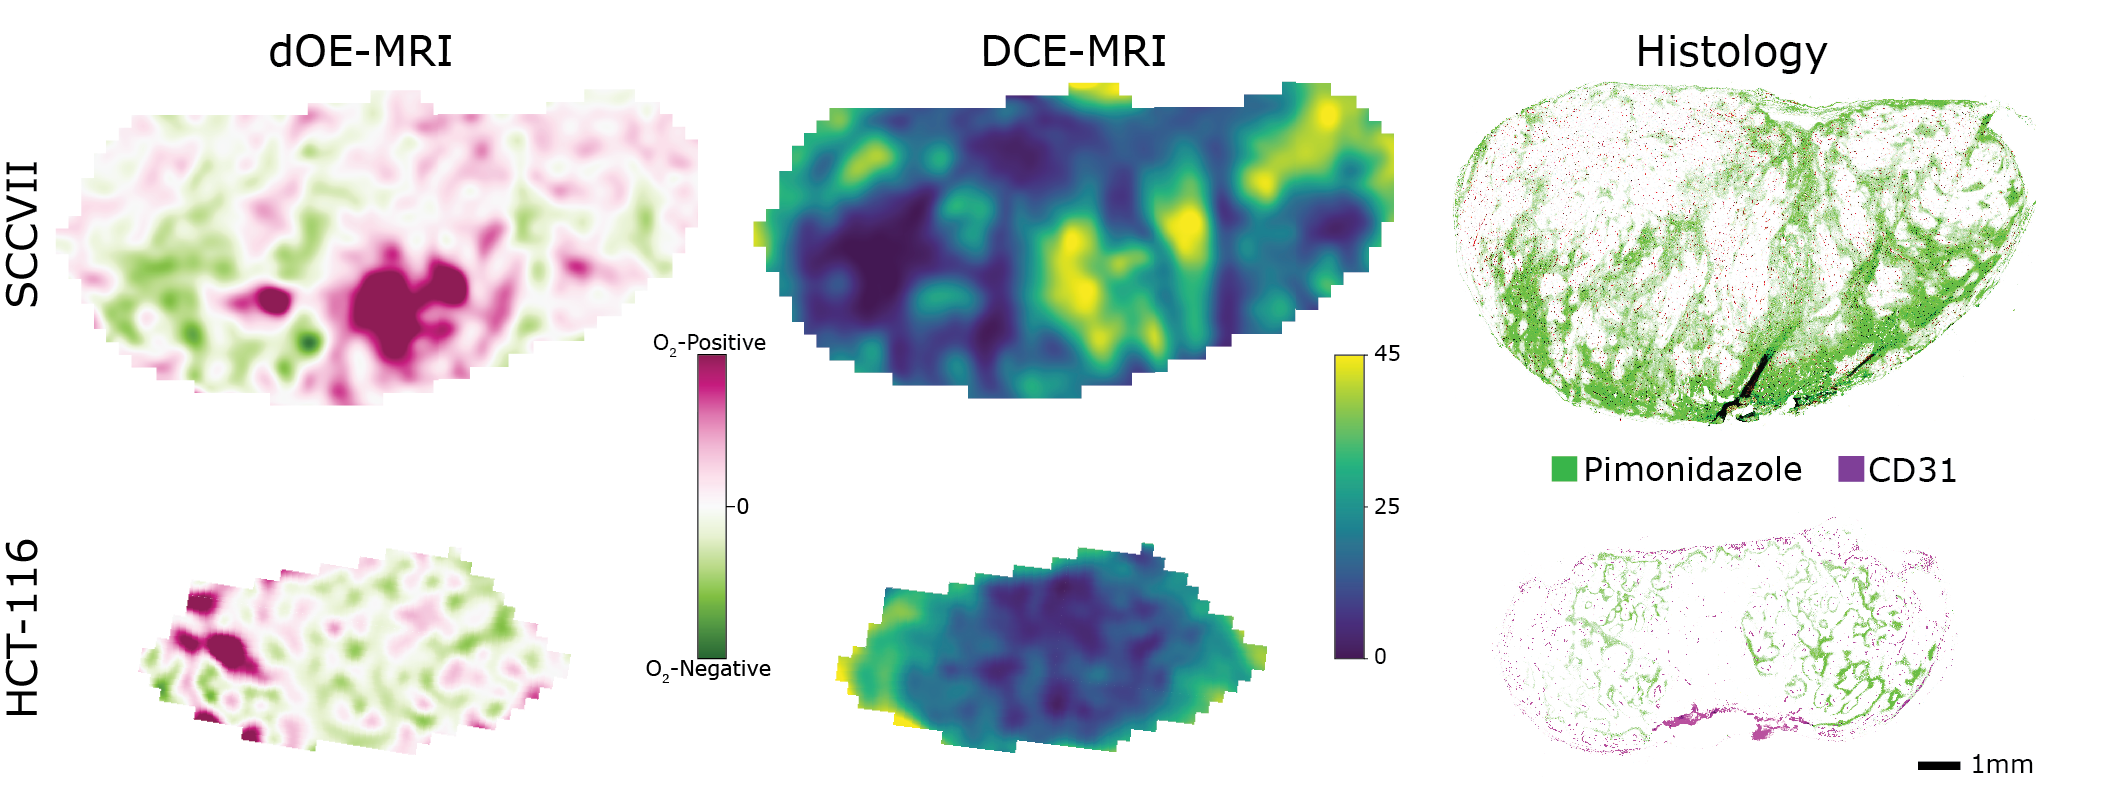
\includegraphics[width=\textwidth]{futurework/futurework-images/fig_perfusion.pdf} % requires the graphicx package
   \caption{\ac{dOE-MRI} maps and DCE-MRI IAUC$_{60}$maps and slice-matched histology sections of SCCVII and HCT-116 tumours. Large regions marked as purple in the \ac{dOE-MRI} maps are O$_2$-positive and also correspond to regions that have high IAUC$_{60}$ values (yellow). Green or O$_2$-negative regions from the \ac{dOE-MRI} map are often consistent with unperfused regions in the IAUC$_{60}$ (black), but there are regions of mismatch. Histology images stained with pimonidazole (green) and CD31 (purple) are shown for corresponding sections.
   \label{fig_perfusion}}
\end{figure}


\begin{figure}[htbp]
   \centering
   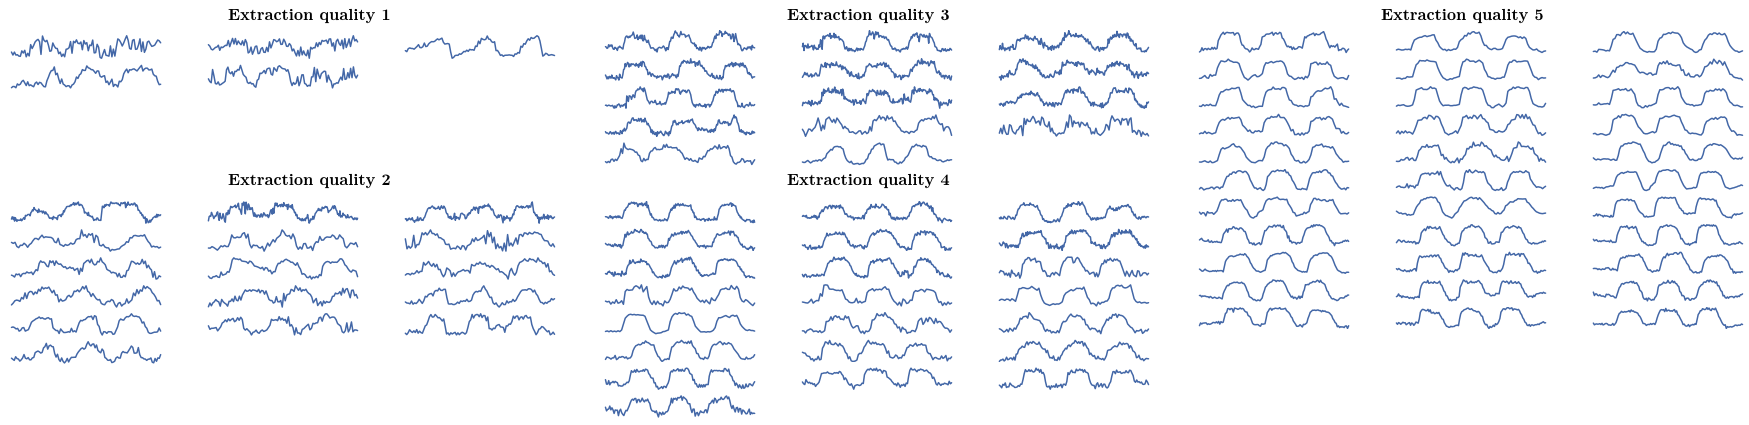
\includegraphics[width=\textwidth]{futurework/futurework-images/technical_ScoredExtractions.png} % requires the graphicx package
   \caption{Each trace plot is the extracted ICA component corresponding to the oxygen response. The components are scored by the observer from a score of 1 to 5, with 1 barely corresponding to the oxygen challenge with a lot of noise and 5 corresponding extremely well to the oxygen challenge and very little noise. Note very few animals are in the lowest group, and many more are of extraction quality 4 and 5.}
   \label{extractions}
\end{figure}





\endinput